\begin{center}
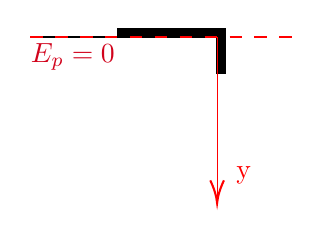
\begin{tikzpicture}[x=0.75pt,y=0.75pt,yscale=-1,xscale=1]
%uncomment if require: \path (0,300); %set diagram left start at 0, and has height of 300

%Straight Lines [id:da9215028484159156] 
\draw    (160,110) -- (250,110) -- (250,180) ;
%Straight Lines [id:da4977009583781107] 
\draw [line width=3.75]    (202,108) -- (252,108) -- (252,128) ;
%Straight Lines [id:da23325832635314958] 
\draw [color={rgb, 255:red, 255; green, 0; blue, 0 }  ,draw opacity=1 ]   (250,110) -- (250,188) ;
\draw [shift={(250,190)}, rotate = 270] [color={rgb, 255:red, 255; green, 0; blue, 0 }  ,draw opacity=1 ][line width=0.75]    (10.93,-3.29) .. controls (6.95,-1.4) and (3.31,-0.3) .. (0,0) .. controls (3.31,0.3) and (6.95,1.4) .. (10.93,3.29)   ;
%Straight Lines [id:da8953033878619383] 
\draw [color={rgb, 255:red, 255; green, 0; blue, 0 }  ,draw opacity=1 ] [dash pattern={on 4.5pt off 4.5pt}]  (160,110) -- (290,110) ;

% Text Node
\draw (258,171) node [anchor=north west][inner sep=0.75pt]  [color={rgb, 255:red, 255; green, 0; blue, 0 }  ,opacity=1 ] [align=left] {y};
% Text Node
\draw (159,112) node [anchor=north west][inner sep=0.75pt]   [align=left] {$\displaystyle \textcolor[rgb]{0.82,0.01,0.11}{E_{p} =0}$};
\end{tikzpicture}
\end{center}